\documentclass[a4paper,11pt]{article}
\usepackage[spanish]{babel}
\usepackage{amsmath, amssymb}
\usepackage{graphicx}
\usepackage[utf8]{inputenc}
\usepackage{amsfonts}
\usepackage{stmaryrd}

\title{Resumen: Lenguaje Imperativo Simple (LIS)}
\author{}
\date{}

\begin{document}

\maketitle

\section{Lenguaje Imperativo Simple (LIS)}

\subsection{Gramática abstracta}

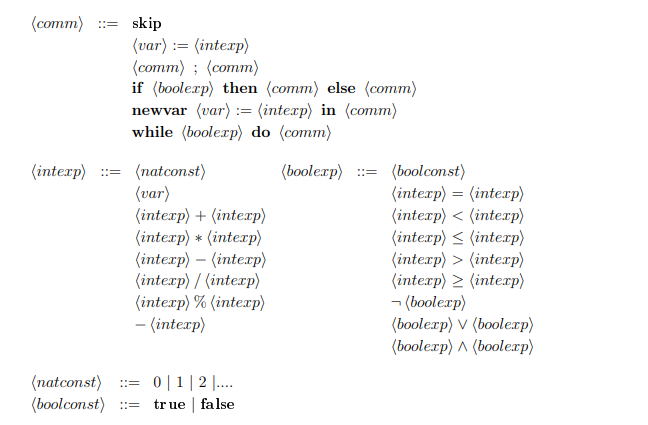
\includegraphics[width=1\textwidth]{./gramaticaAbstractaLIS}

\subsection{Estados}

\[
\Sigma = \text{Var} \to \mathbb{Z}
\]

Un estado es una función que asigna a cada variable un entero.

\section{Funciones semánticas}

\begin{align*}
[\![\cdot]\!]_{intexp} &: \langle intexp \rangle \to (\Sigma \to \mathbb{Z}) \\
[\![\cdot]\!]_{boolexp} &: \langle boolexp \rangle \to (\Sigma \to \{V,F\}) \\
[\![\cdot]\!]_{comm} &: \langle comm \rangle \to (\Sigma \to \Sigma)
\end{align*}
\text{Todos los comandos terminan en su ejecución y su "resultado" es un nuevo estado}

\section{Problema de la iteración}

\subsection{No terminación}

Se introduce:
\[
\Sigma_\bot = \Sigma \cup \{\bot\}
\]

\subsection{Nuevo tipo semántico}

\[
[\![\cdot]\!] : \langle comm \rangle \to (\Sigma \to \Sigma_\bot)
\]

\section{Extensión estricta}

Dada una $f \in P \to D$, donde $P$ es un predominio y $D$ un dominio, se denota por $f_{\bot\bot}$ la única extensión estricta de $f$ a $P_{\bot}$. Así, $f_{\bot\bot} \in P_{\bot} \to D$ está definida por:

$$f_{\bot\bot} \, x = 
\begin{cases} 
\bot & \text{si } x = \bot \\
f \, x & \text{si no}
\end{cases}$$

\section{Resumen de llaves semanticas}

\subsection*{Expresiones Enteras}
$\llbracket \cdot \rrbracket \in \langle intexp \rangle \rightarrow \Sigma \rightarrow \mathbb{Z}$
\begin{align*}
    \llbracket 0 \rrbracket \sigma &= 0 \\
    \llbracket -e \rrbracket \sigma &= -\llbracket e \rrbracket \sigma \\
    \llbracket e_0 + e_1 \rrbracket \sigma &= \llbracket e_0 \rrbracket \sigma + \llbracket e_1 \rrbracket \sigma \quad \text{(similarmente para $-, *, \dots$)} \\
    \llbracket v \rrbracket \sigma &= \sigma \, v
\end{align*}

\subsection*{Expresiones Booleanas}
$\llbracket \cdot \rrbracket \in \langle boolexp \rangle \rightarrow \Sigma \rightarrow \mathbb{B}$
\begin{align*}
    \llbracket \text{true} \rrbracket \sigma &= V \\
    \llbracket \text{false} \rrbracket \sigma &= F \\
    \llbracket e_0 = e_1 \rrbracket \sigma &= \llbracket e_0 \rrbracket \sigma = \llbracket e_1 \rrbracket \sigma \quad \text{(similarmente para $<, >, \dots$)} \\
    \llbracket \neg b \rrbracket \sigma &= \neg \llbracket b \rrbracket \sigma \\
    \llbracket b_0 \wedge b_1 \rrbracket \sigma &= \llbracket b_0 \rrbracket \sigma \wedge \llbracket b_1 \rrbracket \sigma \quad \text{(similarmente para $\vee, \dots$)}
\end{align*}

\subsection*{Comandos}
$\llbracket \cdot \rrbracket \in \langle comm \rangle \rightarrow \Sigma \rightarrow \Sigma_\perp$
\begin{align*}
    \llbracket \text{skip} \rrbracket \sigma &= \sigma \\
    \llbracket v := e \rrbracket \sigma &= [\sigma | v : \llbracket e \rrbracket \sigma] \\
    \llbracket \text{if } b \text{ then } c_0 \text{ else } c_1 \rrbracket \sigma &= 
    \begin{cases} 
        \llbracket c_0 \rrbracket \sigma & \text{si } \llbracket b \rrbracket \sigma \\ 
        \llbracket c_1 \rrbracket \sigma & \text{si no} 
    \end{cases} \\
    \llbracket c_0; c_1 \rrbracket \sigma &= \llbracket c_1 \rrbracket_\perp (\llbracket c_0 \rrbracket \sigma) \\
    \llbracket \text{newvar } v := e \text{ in } c \rrbracket \sigma &= (\lambda \sigma' \in \Sigma. [\sigma' | v : \sigma \, v])_\perp (\llbracket c \rrbracket [\sigma | v : \llbracket e \rrbracket \sigma]) \\
    \llbracket \text{while } b \text{ do } c \rrbracket &= \bigsqcup_{i=0}^{\infty} F^i \perp_{\Sigma \rightarrow \Sigma_\perp}
\end{align*}

\noindent donde:
\begin{align*}
    f_{\perp\perp} x &= \begin{cases} \perp & \text{si } x = \perp \\ f \, x & \text{si no} \end{cases} \\
    F \, w \, \sigma &= \begin{cases} w_{\perp\perp} (\llbracket c \rrbracket \sigma) & \text{si } \llbracket b \rrbracket \sigma \\ \sigma & \text{si no} \end{cases}
\end{align*}

\section{Propiedades}

\subsection{Variables libres}

\begin{align*}
FV(\texttt{skip}) &= \emptyset \\
FV(v := e) &= \{v\} \cup FV(e) \\
FV(c_0 ; c_1) &= FV(c_0) \cup FV(c_1) \\
FV(\texttt{if } b \texttt{ then } c_0 \texttt{ else } c_1) &= FV(b) \cup FV(c_0) \cup FV(c_1) \\
FV(\texttt{while } b \texttt{ do } c) &= FV(b) \cup FV(c) \\
FV(\texttt{newvar } v := e \texttt{ in } c) &= FV(e) \cup (FV(c) - \{v\})
\end{align*}

\subsection{Variables asignables}

\begin{align*}
FA(\texttt{skip}) &= \emptyset \\
FA(v := e) &= \{v\} \\
FA(c_0 ; c_1) &= FA(c_0) \cup FA(c_1) \\
FA(\texttt{if } b \texttt{ then } c_0 \texttt{ else } c_1) &= FA(c_0) \cup FA(c_1) \\
FA(\texttt{while } b \texttt{ do } c) &= FA(c) \\
FA(\texttt{newvar } v := e \texttt{ in } c) &= FV(c) - \{v\}
\end{align*}

\subsection{Teorema de Coincidencia}

\begin{enumerate}
    \item $(\forall w \in FV(c). \sigma w = \sigma' w)$ implica,
    \begin{itemize}
        \item o bien $\llbracket c \rrbracket \sigma = \bot = \llbracket c \rrbracket \sigma'$,
        \item o bien $\llbracket c \rrbracket \sigma \neq \bot \neq \llbracket c \rrbracket \sigma'$ y $\forall w \in FV(c). \llbracket c \rrbracket \sigma w = \llbracket c \rrbracket \sigma' w$
    \end{itemize}
    \item Si $\llbracket c \rrbracket \sigma \neq \bot$, entonces $\forall w \notin FA(c). \llbracket c \rrbracket \sigma w = \sigma w$. (esto es intangibilidad)
\end{enumerate}

\subsection{Teorema de Renombre}
Otra propiedad que cobra importancia en el lenguaje imperativo es la que establece que no importa el nombre de las variables utilizadas en las declaraciones de variables locales (o sea las ligadas):

$$u \notin FV(c) - \{v\} \Rightarrow \llbracket \textbf{newvar } u := e \textbf{ in } c[v \to u] \rrbracket = \llbracket \textbf{newvar } v := e \textbf{ in } c \rrbracket$$

\section{Sustituciones}
Conjunto de sustituciones
\[
\Delta = \text{Var} \to \text{Var}
\]

Las ecuaciones que la definían para la lógica de predicados siguen valiendo (salvo el caso de los cuantificadores, que ahora no tenemos). Ahora se agregan ecuaciones para los comandos.

$$\_ / \_ \in \langle comm \rangle \times \Delta \to \langle comm \rangle$$

\begin{align*}
    \textbf{skip} / \delta &= \textbf{skip} \\
    (v := e) / \delta &= (\delta v) := (e / \delta) \\
    (c_0 ; c_1) / \delta &= (c_0 / \delta) ; (c_1 / \delta) \\
    (\textbf{if } b \textbf{ then } c_0 \textbf{ else } c_1) / \delta &= \textbf{if } b / \delta \textbf{ then } c_0 / \delta \textbf{ else } c_1 / \delta \\
    (\textbf{while } b \textbf{ do } c) / \delta &= \textbf{while } b / \delta \textbf{ do } c / \delta
\end{align*}

El caso del \textbf{newvar} tiene los mismos inconvenientes que los cuantificadores, ahora es un poco más simple ya que $\delta w$ son siempre variables.

$$(\textbf{newvar } v := e \textbf{ in } c) / \delta = \textbf{newvar } v_{new} := e / \delta \textbf{ in } (c / [\delta | v : v_{new}])$$

donde $v_{new} \notin \{ \delta w | w \in FV(c) - \{v\} \}$

\subsection{Teorema de Sustitución}

Si $\delta$ es inyectiva sobre $FV(c)$ y $\forall w \in FV(c). \ \sigma(\delta w) = \sigma' w$, entonces
\begin{itemize}
    \item o bien $\llbracket c/\delta \rrbracket \sigma = \bot = \llbracket c \rrbracket \sigma'$,
    \item o bien $\llbracket c/\delta \rrbracket \sigma \neq \bot \neq \llbracket c \rrbracket \sigma'$ y $\forall w \in FV(c). \ \llbracket c/\delta \rrbracket \sigma(\delta w) = \llbracket c \rrbracket \sigma' w$.
\end{itemize}

\subsection{Lema de Sustitución}
Sea $FV(c) \subseteq V \subseteq \langle var \rangle$ tal que $\delta$ es inyectiva sobre $V$ y $\forall w \in V. \ \sigma(\delta w) = \sigma' w$. Entonces,
\begin{itemize}
    \item o bien $\llbracket c/\delta \rrbracket \sigma = \bot = \llbracket c \rrbracket \sigma'$,
    \item o bien $\llbracket c/\delta \rrbracket \sigma \neq \bot \neq \llbracket c \rrbracket \sigma'$ y $\forall w \in V. \ \llbracket c/\delta \rrbracket \sigma(\delta w) = \llbracket c \rrbracket \sigma' w$.
\end{itemize}

\section{Fallas en el Lenguaje Imperativo Simple}

Para modelar la transferencia de control por fallas, se incorporan excepciones al lenguaje imperativo mediante nuevas construcciones:

\[
\langle comm \rangle ::= fail \mid catchin \ \langle comm \rangle \ with \ \langle comm \rangle
\]

\subsection{Dominio semántico}

Se extiende el conjunto de estados:
\[
\Sigma' = \Sigma \cup (\{abort\} \times \Sigma)
\]

La función semántica queda definida como:
\[
[[\_]] : \langle comm \rangle \to (\Sigma \to \Sigma'_\bot)
\]

donde $\Sigma'_\bot$ es un dominio llano con elemento indefinido $\bot$.

\subsection{Semántica de los comandos básicos}

\begin{align*}
[[skip]]\sigma &= \sigma \\
[[fail]]\sigma &= \langle abort, \sigma \rangle \\
[[v := e]]\sigma &= \sigma[v \mapsto [[e]]\sigma]
\end{align*}

\subsection{Operadores de transferencia de control}

Para definir la semántica de composición y manejo de excepciones, se introducen tres operadores:

\begin{itemize}
    \item \textbf{Extensión estricta ($f_*$):} Propaga fallas (no continúa la ejecución).
    \[
    f_*(x) =
    \begin{cases}
    f(\sigma) & \text{si } x = \sigma \in \Sigma \\
    x & \text{si } x \text{ es abort o } \bot
    \end{cases}
    \]

    \item \textbf{Extensión de manejo ($f_+$):} Se ejecuta solo si hubo falla.
    \[
    f_+(x) =
    \begin{cases}
    f(\sigma) & \text{si } x = \langle abort, \sigma \rangle \\
    x & \text{en otro caso}
    \end{cases}
    \]

    \item \textbf{Extensión total ($f_\dagger$):} Se ejecuta siempre, preservando el estado de falla (en este caso se hace asi ya que queremos que en el newvar se ejecute la función para restaurar el estado original).
    \[
    f_\dagger(x) =
    \begin{cases}
    \langle abort, f(\sigma) \rangle & \text{si } x = \langle abort, \sigma \rangle \\
    f(x) & \text{si } x \in \Sigma \\
    \bot & \text{si } x = \bot
    \end{cases}
    \]
\end{itemize}

\subsection{Semántica de las construcciones extendidas}

\[
[[c_0; c_1]]\sigma = [[c_1]]_*([[c_0]]\sigma)
\]

\[
[[catchin \ c_0 \ with \ c_1]]\sigma = [[c_1]]_+([[c_0]]\sigma)
\]

\[
[[newvar \ v := e \ in \ c]]\sigma =
(\lambda \sigma'. \sigma'[v \mapsto \sigma(v)])_\dagger
([[c]](\sigma[v \mapsto [[e]]\sigma]))
\]

\[
[[while \ b \ do \ c]] = \bigsqcup_{i=0}^{\infty} F^i(\bot)
\]
donde
\[
F(w)(\sigma) =
\begin{cases}
w_*([[c]]\sigma) & \text{si } [[b]]\sigma \\
\sigma & \text{en otro caso}
\end{cases}
\]

\section{Entrada/Salida y Manejo de Errores}
\subsection{Sintaxis de Comandos}

\[
\begin{array}{rcl}
\langle comm \rangle & ::= & \text{skip} \mid \langle var \rangle := \langle intexp \rangle \mid \langle comm \rangle ; \langle comm \rangle \\
& \mid & \text{if } \langle boolexp \rangle \text{ then } \langle comm \rangle \text{ else } \langle comm \rangle \\
& \mid & \text{newvar } \langle var \rangle := \langle intexp \rangle \text{ in } \langle comm \rangle \\
& \mid & \text{while } \langle boolexp \rangle \text{ do } \langle comm \rangle \\
& \mid & \text{fail} \mid \text{catchin } \langle comm \rangle \text{ with } \langle comm \rangle \\
& \mid & ! \langle intexp \rangle \mid ? \langle var \rangle
\end{array}
\]

\subsection{Dominio de Salidas ($\Omega$)}

El dominio de salidas $\Omega$ se define como el conjunto de posibles resultados de la ejecución de un programa, incluyendo terminación exitosa, error o divergencia (ejecución infinita).

\[
\begin{aligned}
\Omega = & \quad \{\langle n_0, \dots, n_k, \sigma' \rangle \mid n_i \in \mathbb{Z}, \sigma' \in \hat{\Sigma}\} \\
& \cup \{\langle n_0, \dots, n_k \rangle \mid n_i \in \mathbb{Z}\} \\
& \cup \{\langle n_0, n_1, n_2, n_3, \dots, n_k, \dots \rangle \mid n_i \in \mathbb{Z}\}
\end{aligned}
\]

Donde el conjunto de estados extendido $\hat{\Sigma}$ se define como:
\[
\hat{\Sigma} = \Sigma \cup (\{\mathbf{abort}\} \times \Sigma)
\]

\subsection{Concatenación de tuplas}

Podemos ``concatenar'' ciertos elementos de $\Omega$ para obtener nuevos elementos del mismo dominio:
\[
\langle n_0, \dots, n_k \rangle \mathbin{+\mkern-10mu+} \langle m_0, \dots, s \rangle
= \langle n_0, \dots, n_k, m_0, \dots, s \rangle
\]

Aquí, $s$ puede representar tanto un número entero como un estado (finalizado o fallido).

\subsection{Estructura del Dominio}

Para tratar la semántica de forma denotacional, definimos una estructura de orden sobre $\Omega$:

\begin{enumerate}
    \item \textbf{Orden de prefijo:} El orden está dado por la relación de prefijo. Por ejemplo:
    \[
    \langle 4, 3, 2, 1 \rangle \sqsubseteq \langle 4, 3, 2, 1, \sigma \rangle
    \]

    \item \textbf{Supremo de cadenas no interesantes:} Es simplemente el último elemento de la cadena.

    \item \textbf{Supremo de cadenas interesantes:} Es la tupla (posiblemente infinita) que coincide en todas las posiciones de cada tupla de la cadena.
\end{enumerate}

\paragraph{Observaciones:}
\begin{itemize}
    \item El elemento mínimo está dado por la tupla vacía: $\langle \rangle$.
    \item En una cadena ``interesante'' de tuplas, existen tuplas de cada longitud, por lo tanto, el supremo es efectivamente único.
\end{itemize}

\subsection{Semántica de Programas}

La nueva semántica de los comandos se define como una función que toma un estado inicial y devuelve un elemento del dominio de salidas:
\[
\llbracket \_ \rrbracket : \langle comm \rangle \to (\Sigma \to \Omega)
\]

\subsection{Reglas semánticas}

Para el comando de salida de datos ($!e$):
\[
\llbracket !e \rrbracket \sigma = \langle \llbracket e \rrbracket \sigma, \sigma \rangle
\]
    \[
    \llbracket \mathbf{skip} \rrbracket \sigma = \langle \sigma \rangle
    \]
    \[
    \llbracket v := e \rrbracket \sigma = \langle \sigma [v : \llbracket e \rrbracket \sigma] \rangle
    \]
    \[
    \llbracket \mathbf{if} \ b \ \mathbf{then} \ c \ \mathbf{else} \ c' \rrbracket \sigma =
    \begin{cases}
        \llbracket c \rrbracket \sigma & \text{si } \llbracket b \rrbracket \sigma \\
        \llbracket c' \rrbracket \sigma & \text{si } \neg \llbracket b \rrbracket \sigma
    \end{cases}
    \]
    \[
    \llbracket c_0; c_1 \rrbracket \sigma =
    \llbracket c_1 \rrbracket_{*} (\llbracket c_0 \rrbracket \sigma)
    \]
    \[
    \llbracket \mathbf{newvar} \ v := e \ \mathbf{in} \ c \rrbracket \sigma =
    (rest_{v,\sigma})_{\dagger} \left( \llbracket c \rrbracket [\sigma \mid v : \llbracket e \rrbracket \sigma] \right)
    \]

\subsection{Semántica del Bucle (While)}
\[
F_{b,c} : (\Sigma \to \Sigma') \to (\Sigma \to \Sigma')
\]

\[
F_{b,c}(f)(\sigma) =
\begin{cases}
    \sigma & \text{si } \neg \llbracket b \rrbracket \sigma \\
    f_{*} (\llbracket c \rrbracket \sigma) & \text{si } \llbracket b \rrbracket \sigma
\end{cases}
\]

\[
\llbracket \mathbf{while} \ b \ \mathbf{do} \ c \rrbracket \sigma =
\left( \bigsqcup_{i \in \mathbb{N}} F^i \perp \right) \sigma
\]

\paragraph{Nota:}
No es necesario cambiar la estructura de la ecuación, solo redefinir adecuadamente los operadores ($*$, $\dagger$, $\sqcup$) sobre el nuevo dominio $\Omega$.

\section{Funciones de Propagación de Errores}

Estas funciones definen cómo se comportan las transformaciones de estado cuando encuentran estados de error o terminación.

\subsection{Propagación estándar $(\_)_{*}$}

La función $(\_)_{*}$ extiende una función de estado a una que maneja errores y abortos:
\[
(\_)_{*} : (\Sigma \to \Sigma') \to (\Sigma' \to \Sigma')
\]

\[
\begin{aligned}
f_{*}(\perp) &= \perp \\
f_{*}(\langle \mathbf{abort}, \sigma \rangle) &= \langle \mathbf{abort}, \sigma \rangle \\
f_{*}(\sigma) &= f(\sigma)
\end{aligned}
\]

\subsection{Propagación tipo Map $(\_)_{\dagger}$}

Similar a la función \texttt{map} en listas, aplica una transformación incluso en estados de aborto:
\[
(\_)_{\dagger} : (\Sigma \to \Sigma) \to (\Sigma' \to \Sigma')
\]

\[
\begin{aligned}
f_{\dagger}(\perp) &= \perp \\
f_{\dagger}(\langle \mathbf{abort}, \sigma \rangle) &= \langle \mathbf{abort}, f(\sigma) \rangle \\
f_{\dagger}(\sigma) &= f(\sigma)
\end{aligned}
\]

\section{Revisión de Funciones sobre $\Omega$}

Al trabajar con el dominio de secuencias $\Omega$, las funciones de propagación se redefinen para operar sobre tuplas de enteros y estados.

\subsection{Propagación en $\Omega$}

\[
(\_)_{*} : (\Sigma \to \Omega) \to (\Omega \to \Omega)
\]

\[
\begin{aligned}
f_{*}(\langle n_0, \dots, n_{k-1} \rangle) &= \langle n_0, \dots, n_{k-1} \rangle \\
f_{*}(\langle n_0, \dots, n_{k-1}, \sigma \rangle) &= \langle n_0, \dots, n_{k-1} \rangle \mathbin{+\mkern-10mu+} f(\sigma) \\
f_{*}(\langle n_0, \dots, n_{k-1}, \langle \mathbf{abort}, \sigma \rangle \rangle) &= \langle n_0, \dots, n_{k-1}, \langle \mathbf{abort}, \sigma \rangle \rangle \\
f_{*}(\langle n_0, \dots, n_{k-1}, \dots \rangle) &= \langle n_0, \dots, n_{k-1}, \dots \rangle
\end{aligned}
\]

\subsection{Función Map en $\Omega$}

\[
(\_)_{\dagger} : (\Sigma \to \Sigma) \to (\Omega \to \Omega)
\]

\[
\begin{aligned}
f_{\dagger}(\langle n_0, \dots, n_{k-1} \rangle) &= \langle n_0, \dots, n_{k-1} \rangle \\
f_{\dagger}(\langle n_0, \dots, n_{k-1}, \sigma \rangle) &= \langle n_0, \dots, n_{k-1}, f(\sigma) \rangle \\
f_{\dagger}(\langle n_0, \dots, n_{k-1}, \langle \mathbf{abort}, \sigma \rangle \rangle) &= \langle n_0, \dots, n_{k-1}, \langle \mathbf{abort}, f(\sigma) \rangle \rangle \\
f_{\dagger}(\langle n_0, \dots, n_{k-1}, \dots \rangle) &= \langle n_0, \dots, n_{k-1}, \dots \rangle
\end{aligned}
\]

\section{Funciones Inyectoras y Constructores}

Para facilitar la definición recursiva de la semántica, consideramos las siguientes funciones auxiliares:

\[
\begin{aligned}
\iota_{\perp} &: \{\langle \rangle\} \to \Omega 
& \iota_{term} &: \Sigma \to \Omega \\
\iota_{\perp}(\langle \rangle) &= \langle \rangle 
& \iota_{term}(\sigma) &= \langle \sigma \rangle \\
\iota_{abort} &: \Sigma \to \Omega 
& \iota_{out} &: \mathbb{Z} \times \Omega \to \Omega \\
\iota_{abort}(\sigma) &= \langle \sigma \rangle 
& \iota_{out}(\langle n, \omega \rangle) &= \langle n \rangle \mathbin{+\mkern-10mu+} \omega
\end{aligned}
\]

\subsection{Propagación de errores (Definición Alternativa)}

Utilizando los constructores anteriores, la propagación $f_{*}$ se puede ver como:

\[
\begin{aligned}
f_{*}(\perp) &= \perp \\
f_{*}(\iota_{term}(\sigma)) &= f(\sigma) \\
f_{*}(\iota_{abort}(\sigma)) &= \iota_{abort}(\sigma) \\
f_{*}(\iota_{out}(\langle n, \omega \rangle)) &= \iota_{out}(\langle n, f_{*}(\omega) \rangle)
\end{aligned}
\]

\paragraph{Observación:}
Para asegurar que el mínimo punto fijo exista y sea único, es fundamental que la función $f_{*}$ sea \textbf{continua}.

\end{document}